 % Created 2021-11-03 mié 11:39
% Intended LaTeX compiler: lualatex
\documentclass[table]{scrartcl}
\usepackage[left=1.5cm,right=1.5cm,bottom=2.5cm,letterpaper]{geometry}
\usepackage[spanish, es-nodecimaldot, es-tabla]{babel}
\usepackage[utf8]{inputenc}
\usepackage{blindtext}
\usepackage{multicol}
\usepackage{subfigure}
\usepackage[most]{tcolorbox}
\usepackage{etoolbox}
\usepackage{minted}
\usepackage{hyperref}
% \usepackage[table,xcdraw]{xcolor}
\usepackage{longtable}
\usepackage{multirow}
\usepackage[default]{comfortaa}
\usepackage[T1]{fontenc}

\usepackage{caption}
\usepackage{breqn}
\usemintedstyle{emacs}
\usepackage[ruled,vlined]{algorithm2e}
\newenvironment{code}{\captionsetup{type=listing}}{}
\definecolor{custom}{HTML}{F8F8F8}
\setminted{frame=lines,breaklines=true,bgcolor=custom,fontsize=\scriptsize,linenos}
\renewcommand\listoflistingscaption{Índice de \listingscaption\@s}
\renewcommand{\listingscaption}{Código}
\BeforeBeginEnvironment{listing}{\begin{code}}
  \AfterEndEnvironment{listing}{\end{code}}
\BeforeBeginEnvironment{minted}{\begin{code}}
  \AfterEndEnvironment{minted}{\end{code}}
\author{Monsalvo Bolaños Melissa Monserrat y Romero Andrade Cristian}
\date{\today}
\title{Practica 5}
\hypersetup{
  pdfauthor={Monsalvo Bolaños Melissa Monserrat y Romero Andrade Cristian},
  pdftitle={Practica 5},
  pdfkeywords={},
  pdfsubject={},
  pdfcreator={Emacs 27.2 (Org mode 9.6)},
  pdflang={English}}

\newcommand{\tituloTrabajo}{Práctica No 5\\Construcción de
Máquinas de estados Usando Memorias
Direccionamiento Implícito}
\newcommand{\fechaEntrega}{21 de octubre de 2021}

\usepackage{subfiles}
\usepackage[backend=biber,style=apa]{biblatex}
\addbibresource{../bib.bib}

\begin{document}
\begin{titlepage}
  \centering

    {\scshape{\Huge Facultad de Ingeniería\par{}}}\vspace{0.25cm}

    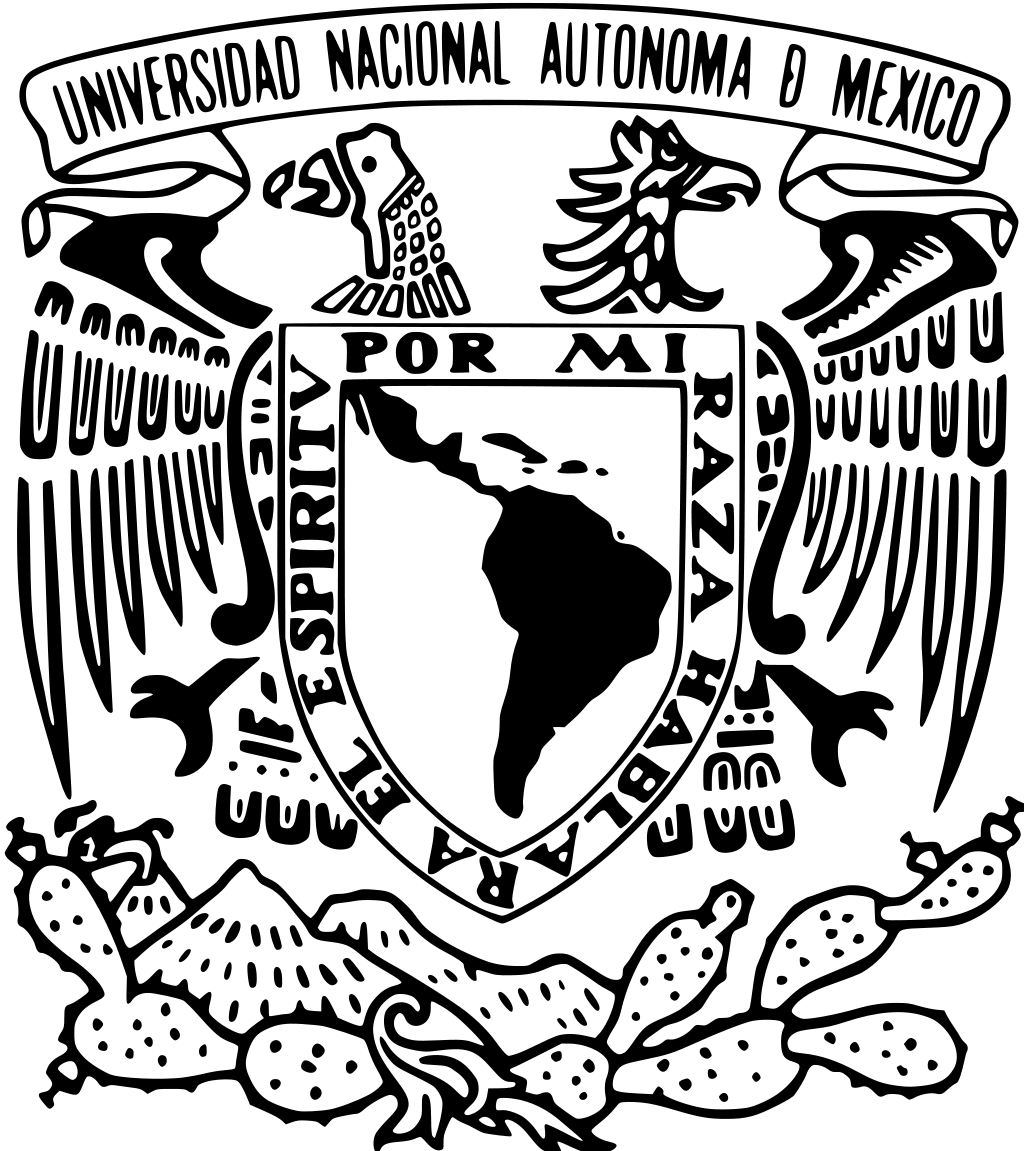
\includegraphics[width=0.25\textwidth]{../img_common/unam_logo}\vspace{0.5cm}

    {\scshape{\Large Lab. Organización y Arquitectura de Computadoras\par{}}}\vfill{}


    {\huge \textbf{\tituloTrabajo{}}}\vfill{}


    {\Large
      Alumnos
      \begin{itemize}

        \item Monsalvo Bolaños Melissa Monserrat

        \item Romero Andrade Cristian
      \end{itemize}
    }\vfill{}

      {\large Grupo: 01\par{}}\vfill{}

    {\large Profesor\\Ing.~Adrian Ulises Mercado Martinez}\vfill{}
    \vfil{}
    {\large Semestre\\\textbf{2022--1}}
    \vfill{}
    % {\large Fecha de Entrega\\\fechaEntrega}
    % \vfill{}
    
\includegraphics[width=0.1\textwidth]{../img_common/inge_logo}

\end{titlepage}

\date{}
\maketitle{}
\tableofcontents{}
\section{Introducción}
Este tipo de direccionamiento utiliza solamente un campo de liga. Una variable
de entrada seleccionada por el campo de prueba, y VF, son las que deciden si se
utiliza la dirección de liga (se carga el valor de liga en el contador) o no (se
incrementa el contador en una unidad). El campo VF (Verdadero-Falso) sirve para
indicarle a la lógica cuánto debe valer la variable de entrada, para así cargar
en el contador el valor de la liga y hacer el salto.
\begin{figure}[htbp]
  \centering
  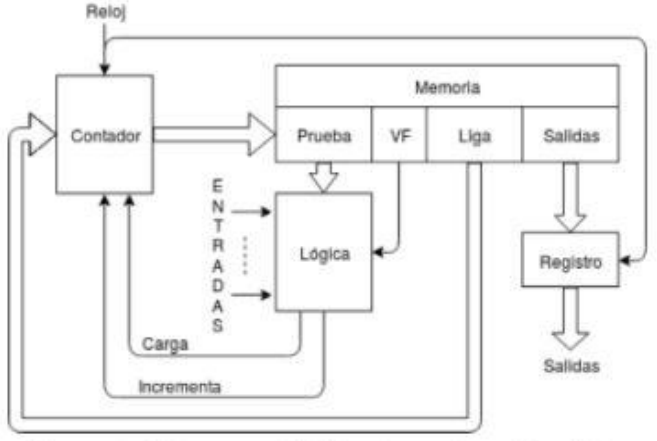
\includegraphics[width=0.4\textwidth]{./img/1.png}
  \caption{Diagrama de direccionamiento implícito}\label{fig:1}
\end{figure}
El campo de verdadero-falso (VF) tiene la utilidad de indicar el calo de la
variable de entrada con el objetivo de cargar el contador el valor de la liga y
realizar el salto.
\begin{figure}[htbp]
  \centering
  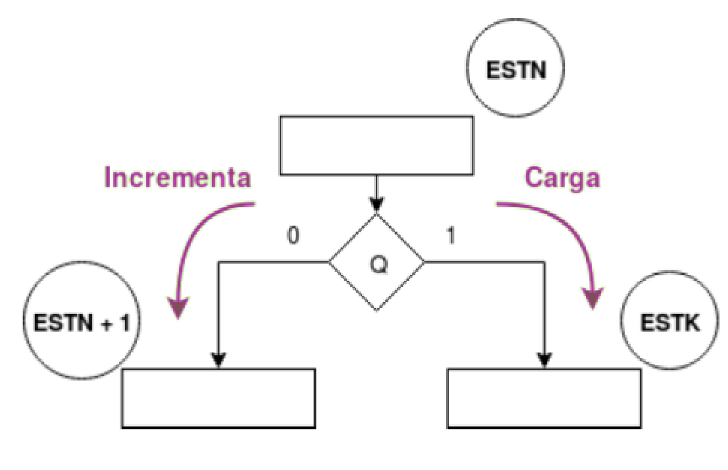
\includegraphics[width=0.4\textwidth]{./img/2.png}
  \caption{Direccionamiento Implicito.}\label{fig:2}
\end{figure}
En la tabla~\ref{tab:1}  muestra la relación de VF y la variable de entrada con
cadenas de incremento y carga
\begin{table}
  \centering
  \caption{Relación VF y Q}\label{tab:1}
  \begin{tabular}{|cc|c|c|}
    \hline
    VF & Q & Incrementa & Carga \\ \hline
    0 & 0 & 0 & 1 \\
    0 & 1 & 1 & 0 \\
    1 & 0 & 1 & 0 \\
    1 & 1 & 0 & 1 \\ \hline
  \end{tabular}
\end{table}
No obstante el diseño original no esta diseño para aceptar salidas
condicionales, es por ello que se propone las siguiente forma.
\begin{figure}[htbp]
  \centering
  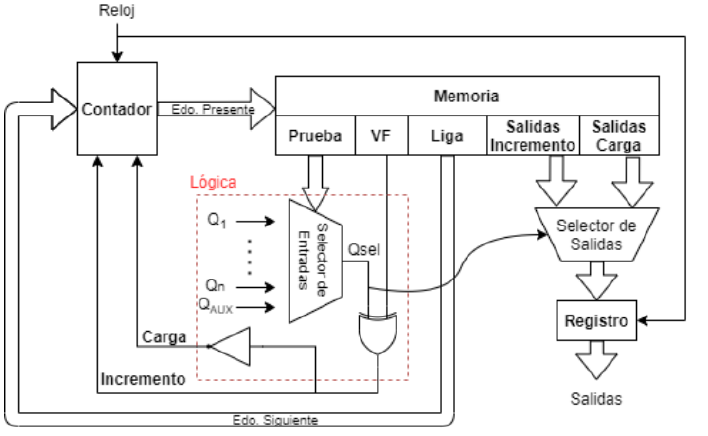
\includegraphics[width=0.6\textwidth]{./img/3.png}
  \caption{Diagrama Modificado}\label{fig:3}
\end{figure}

\section{Objetivo}\label{sec:org8bfa7f0}
Familiarizar al alumno en el conocimiento de construcción de máquinas de estados
usando direccionamiento de memorias con el método de direccionamiento implícito.
\newpage{}
\section{Desarrollo}\label{sec:orgac7043c}
Partimos del análisis de la carta Asm
\begin{figure}[htbp]
  \centering
  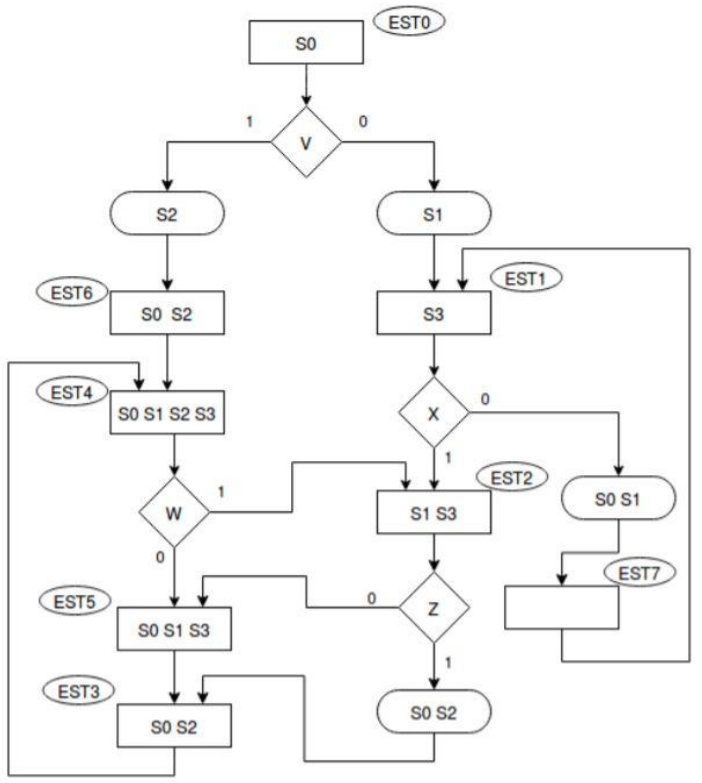
\includegraphics[width=0.6\textwidth]{./img/4.png}
  \caption{Carta ASM}\label{fig:4}
\end{figure}
Asignamos a cada entrada y estado un valor binario
\begin{table}[H]
  \centering
  \caption{Valores binarios deestados}
\begin{tabular}{|c|ccc|}
\hline
\multicolumn{1}{|l|}{Estado} & \multicolumn{3}{l|}{Código binario} \\ \hline
\rowcolor[HTML]{FFE599}
0 & \multicolumn{1}{c|}{\cellcolor[HTML]{FFE599}0} & \multicolumn{1}{c|}{\cellcolor[HTML]{FFE599}0} & 0 \\ \hline
\rowcolor[HTML]{B6D7A8}
1 & \multicolumn{1}{c|}{\cellcolor[HTML]{B6D7A8}0} & \multicolumn{1}{c|}{\cellcolor[HTML]{B6D7A8}0} & 1 \\ \hline
\rowcolor[HTML]{A2C4C9}
2 & \multicolumn{1}{c|}{\cellcolor[HTML]{A2C4C9}0} & \multicolumn{1}{c|}{\cellcolor[HTML]{A2C4C9}1} & 0 \\ \hline
\rowcolor[HTML]{A4C2F4}
3 & \multicolumn{1}{c|}{\cellcolor[HTML]{A4C2F4}0} & \multicolumn{1}{c|}{\cellcolor[HTML]{A4C2F4}1} & 1 \\ \hline
\rowcolor[HTML]{9FC5E8}
4 & \multicolumn{1}{c|}{\cellcolor[HTML]{9FC5E8}1} & \multicolumn{1}{c|}{\cellcolor[HTML]{9FC5E8}0} & 0 \\ \hline
\rowcolor[HTML]{B4A7D6}
5 & \multicolumn{1}{c|}{\cellcolor[HTML]{B4A7D6}1} & \multicolumn{1}{c|}{\cellcolor[HTML]{B4A7D6}0} & 1 \\ \hline
\rowcolor[HTML]{D5A6BD}
6 & \multicolumn{1}{c|}{\cellcolor[HTML]{D5A6BD}1} & \multicolumn{1}{c|}{\cellcolor[HTML]{D5A6BD}1} & 0 \\ \hline
\rowcolor[HTML]{D9D2E9}
7 & \multicolumn{1}{c|}{\cellcolor[HTML]{D9D2E9}1} & \multicolumn{1}{c|}{\cellcolor[HTML]{D9D2E9}1} & 1 \\ \hline
\end{tabular}
\end{table}
\begin{table}[H]
  \centering
\caption{Valores binarios de variables}
\begin{tabular}{cccc}
\rowcolor[HTML]{E6B8AF}
v & 0 & 0 & 0 \\
\rowcolor[HTML]{F4CCCC}
w & 0 & 0 & 1 \\
\rowcolor[HTML]{FCE5CD}
x & 0 & 1 & 0 \\
\rowcolor[HTML]{FFF2CC}
z & 0 & 1 & 1 \\
\rowcolor[HTML]{D9EAD3}
aux & 1 & 0 & 0
\end{tabular}
\end{table}
Posteriormente rellenamos la tabla de verdad conforme a la carta ASM
\begin{center}
  \captionof{table}{Tabla de verdad de la carta ASM}
  \begin{longtable}{|ccc|ccccccccccccccccccc|}
\hline
\rowcolor[HTML]{CC4125}
\multicolumn{3}{|c|}{\cellcolor[HTML]{CC4125}{\color[HTML]{FFFFFF} \textbf{Dirección de memoria}}} & \multicolumn{19}{c|}{\cellcolor[HTML]{CC4125}Contenido de la memoria} \\ \hline
\rowcolor[HTML]{E06666}
\multicolumn{3}{|c|}{\cellcolor[HTML]{E06666}Estado Presente} & \multicolumn{3}{c|}{\cellcolor[HTML]{E06666}} & \multicolumn{3}{c|}{\cellcolor[HTML]{E06666}} & \multicolumn{3}{c|}{\cellcolor[HTML]{E06666}} & \multicolumn{5}{c|}{\cellcolor[HTML]{E06666}Salidas Falsas} & \multicolumn{5}{c|}{\cellcolor[HTML]{E06666}Salidas Verdaderas} \\ \cline{1-3} \cline{13-22}
\rowcolor[HTML]{F6B26B}
\multicolumn{1}{|c|}{\cellcolor[HTML]{F6B26B}Q2} & \multicolumn{1}{c|}{\cellcolor[HTML]{F6B26B}Q1} & Q0 & \multicolumn{3}{c|}{\multirow{-2}{*}{\cellcolor[HTML]{E06666}Prueba}} & \multicolumn{3}{c|}{\multirow{-2}{*}{\cellcolor[HTML]{E06666}Liga Falsa}} & \multicolumn{3}{c|}{\multirow{-2}{*}{\cellcolor[HTML]{E06666}Liga Verdadera}} & \multicolumn{1}{c|}{\cellcolor[HTML]{F6B26B}S5} & \multicolumn{1}{c|}{\cellcolor[HTML]{F6B26B}S3} & \multicolumn{1}{c|}{\cellcolor[HTML]{F6B26B}S2} & \multicolumn{1}{c|}{\cellcolor[HTML]{F6B26B}S1} & \multicolumn{1}{c|}{\cellcolor[HTML]{F6B26B}S0} & \multicolumn{1}{c|}{\cellcolor[HTML]{F6B26B}S5} & \multicolumn{1}{c|}{\cellcolor[HTML]{F6B26B}S3} & \multicolumn{1}{c|}{\cellcolor[HTML]{F6B26B}S2} & \multicolumn{1}{c|}{\cellcolor[HTML]{F6B26B}S1} & S0 \\ \hline
\rowcolor[HTML]{FFE599}
\multicolumn{1}{|c|}{\cellcolor[HTML]{FFE599}0} & \multicolumn{1}{c|}{\cellcolor[HTML]{FFE599}0} & 0 & \multicolumn{1}{c|}{\cellcolor[HTML]{FFE599}1} & \multicolumn{1}{c|}{\cellcolor[HTML]{FFE599}0} & \multicolumn{1}{c|}{\cellcolor[HTML]{FFE599}0} & \multicolumn{1}{c|}{\cellcolor[HTML]{FFE599}0} & \multicolumn{1}{c|}{\cellcolor[HTML]{FFE599}0} & \multicolumn{1}{c|}{\cellcolor[HTML]{FFE599}1} & \multicolumn{1}{c|}{\cellcolor[HTML]{FFE599}0} & \multicolumn{1}{c|}{\cellcolor[HTML]{FFE599}0} & \multicolumn{1}{c|}{\cellcolor[HTML]{FFE599}1} & \multicolumn{1}{c|}{\cellcolor[HTML]{FFE599}0} & \multicolumn{1}{c|}{\cellcolor[HTML]{FFE599}0} & \multicolumn{1}{c|}{\cellcolor[HTML]{FFE599}0} & \multicolumn{1}{c|}{\cellcolor[HTML]{FFE599}0} & \multicolumn{1}{c|}{\cellcolor[HTML]{FFE599}0} & \multicolumn{1}{c|}{\cellcolor[HTML]{FFE599}0} & \multicolumn{1}{c|}{\cellcolor[HTML]{FFE599}0} & \multicolumn{1}{c|}{\cellcolor[HTML]{FFE599}0} & \multicolumn{1}{c|}{\cellcolor[HTML]{FFE599}0} & 0 \\ \hline
\rowcolor[HTML]{B6D7A8}
\multicolumn{1}{|c|}{\cellcolor[HTML]{B6D7A8}0} & \multicolumn{1}{c|}{\cellcolor[HTML]{B6D7A8}0} & 1 & \multicolumn{1}{c|}{\cellcolor[HTML]{B6D7A8}0} & \multicolumn{1}{c|}{\cellcolor[HTML]{B6D7A8}1} & \multicolumn{1}{c|}{\cellcolor[HTML]{B6D7A8}0} & \multicolumn{1}{c|}{\cellcolor[HTML]{B6D7A8}0} & \multicolumn{1}{c|}{\cellcolor[HTML]{B6D7A8}1} & \multicolumn{1}{c|}{\cellcolor[HTML]{B6D7A8}0} & \multicolumn{1}{c|}{\cellcolor[HTML]{B6D7A8}1} & \multicolumn{1}{c|}{\cellcolor[HTML]{B6D7A8}0} & \multicolumn{1}{c|}{\cellcolor[HTML]{B6D7A8}0} & \multicolumn{1}{c|}{\cellcolor[HTML]{B6D7A8}0} & \multicolumn{1}{c|}{\cellcolor[HTML]{B6D7A8}0} & \multicolumn{1}{c|}{\cellcolor[HTML]{B6D7A8}0} & \multicolumn{1}{c|}{\cellcolor[HTML]{B6D7A8}1} & \multicolumn{1}{c|}{\cellcolor[HTML]{B6D7A8}0} & \multicolumn{1}{c|}{\cellcolor[HTML]{B6D7A8}0} & \multicolumn{1}{c|}{\cellcolor[HTML]{B6D7A8}0} & \multicolumn{1}{c|}{\cellcolor[HTML]{B6D7A8}0} & \multicolumn{1}{c|}{\cellcolor[HTML]{B6D7A8}1} & 0 \\ \hline
\rowcolor[HTML]{A2C4C9}
\multicolumn{1}{|c|}{\cellcolor[HTML]{A2C4C9}0} & \multicolumn{1}{c|}{\cellcolor[HTML]{A2C4C9}1} & 0 & \multicolumn{1}{c|}{\cellcolor[HTML]{A2C4C9}1} & \multicolumn{1}{c|}{\cellcolor[HTML]{A2C4C9}0} & \multicolumn{1}{c|}{\cellcolor[HTML]{A2C4C9}0} & \multicolumn{1}{c|}{\cellcolor[HTML]{A2C4C9}0} & \multicolumn{1}{c|}{\cellcolor[HTML]{A2C4C9}1} & \multicolumn{1}{c|}{\cellcolor[HTML]{A2C4C9}1} & \multicolumn{1}{c|}{\cellcolor[HTML]{A2C4C9}0} & \multicolumn{1}{c|}{\cellcolor[HTML]{A2C4C9}1} & \multicolumn{1}{c|}{\cellcolor[HTML]{A2C4C9}1} & \multicolumn{1}{c|}{\cellcolor[HTML]{A2C4C9}0} & \multicolumn{1}{c|}{\cellcolor[HTML]{A2C4C9}0} & \multicolumn{1}{c|}{\cellcolor[HTML]{A2C4C9}0} & \multicolumn{1}{c|}{\cellcolor[HTML]{A2C4C9}0} & \multicolumn{1}{c|}{\cellcolor[HTML]{A2C4C9}0} & \multicolumn{1}{c|}{\cellcolor[HTML]{A2C4C9}0} & \multicolumn{1}{c|}{\cellcolor[HTML]{A2C4C9}0} & \multicolumn{1}{c|}{\cellcolor[HTML]{A2C4C9}0} & \multicolumn{1}{c|}{\cellcolor[HTML]{A2C4C9}0} & 0 \\ \hline
\rowcolor[HTML]{A4C2F4}
\multicolumn{1}{|c|}{\cellcolor[HTML]{A4C2F4}0} & \multicolumn{1}{c|}{\cellcolor[HTML]{A4C2F4}1} & 1 & \multicolumn{1}{c|}{\cellcolor[HTML]{A4C2F4}0} & \multicolumn{1}{c|}{\cellcolor[HTML]{A4C2F4}0} & \multicolumn{1}{c|}{\cellcolor[HTML]{A4C2F4}0} & \multicolumn{1}{c|}{\cellcolor[HTML]{A4C2F4}1} & \multicolumn{1}{c|}{\cellcolor[HTML]{A4C2F4}0} & \multicolumn{1}{c|}{\cellcolor[HTML]{A4C2F4}1} & \multicolumn{1}{c|}{\cellcolor[HTML]{A4C2F4}1} & \multicolumn{1}{c|}{\cellcolor[HTML]{A4C2F4}1} & \multicolumn{1}{c|}{\cellcolor[HTML]{A4C2F4}0} & \multicolumn{1}{c|}{\cellcolor[HTML]{A4C2F4}0} & \multicolumn{1}{c|}{\cellcolor[HTML]{A4C2F4}1} & \multicolumn{1}{c|}{\cellcolor[HTML]{A4C2F4}0} & \multicolumn{1}{c|}{\cellcolor[HTML]{A4C2F4}0} & \multicolumn{1}{c|}{\cellcolor[HTML]{A4C2F4}0} & \multicolumn{1}{c|}{\cellcolor[HTML]{A4C2F4}0} & \multicolumn{1}{c|}{\cellcolor[HTML]{A4C2F4}1} & \multicolumn{1}{c|}{\cellcolor[HTML]{A4C2F4}0} & \multicolumn{1}{c|}{\cellcolor[HTML]{A4C2F4}0} & 0 \\ \hline
\rowcolor[HTML]{9FC5E8}
\multicolumn{1}{|c|}{\cellcolor[HTML]{9FC5E8}1} & \multicolumn{1}{c|}{\cellcolor[HTML]{9FC5E8}0} & 0 & \multicolumn{1}{c|}{\cellcolor[HTML]{9FC5E8}0} & \multicolumn{1}{c|}{\cellcolor[HTML]{9FC5E8}1} & \multicolumn{1}{c|}{\cellcolor[HTML]{9FC5E8}1} & \multicolumn{1}{c|}{\cellcolor[HTML]{9FC5E8}0} & \multicolumn{1}{c|}{\cellcolor[HTML]{9FC5E8}0} & \multicolumn{1}{c|}{\cellcolor[HTML]{9FC5E8}1} & \multicolumn{1}{c|}{\cellcolor[HTML]{9FC5E8}0} & \multicolumn{1}{c|}{\cellcolor[HTML]{9FC5E8}1} & \multicolumn{1}{c|}{\cellcolor[HTML]{9FC5E8}0} & \multicolumn{1}{c|}{\cellcolor[HTML]{9FC5E8}1} & \multicolumn{1}{c|}{\cellcolor[HTML]{9FC5E8}0} & \multicolumn{1}{c|}{\cellcolor[HTML]{9FC5E8}0} & \multicolumn{1}{c|}{\cellcolor[HTML]{9FC5E8}0} & \multicolumn{1}{c|}{\cellcolor[HTML]{9FC5E8}0} & \multicolumn{1}{c|}{\cellcolor[HTML]{9FC5E8}1} & \multicolumn{1}{c|}{\cellcolor[HTML]{9FC5E8}0} & \multicolumn{1}{c|}{\cellcolor[HTML]{9FC5E8}0} & \multicolumn{1}{c|}{\cellcolor[HTML]{9FC5E8}0} & 0 \\ \hline
\rowcolor[HTML]{B4A7D6}
\multicolumn{1}{|c|}{\cellcolor[HTML]{B4A7D6}1} & \multicolumn{1}{c|}{\cellcolor[HTML]{B4A7D6}0} & 1 & \multicolumn{1}{c|}{\cellcolor[HTML]{B4A7D6}1} & \multicolumn{1}{c|}{\cellcolor[HTML]{B4A7D6}0} & \multicolumn{1}{c|}{\cellcolor[HTML]{B4A7D6}0} & \multicolumn{1}{c|}{\cellcolor[HTML]{B4A7D6}0} & \multicolumn{1}{c|}{\cellcolor[HTML]{B4A7D6}1} & \multicolumn{1}{c|}{\cellcolor[HTML]{B4A7D6}1} & \multicolumn{1}{c|}{\cellcolor[HTML]{B4A7D6}0} & \multicolumn{1}{c|}{\cellcolor[HTML]{B4A7D6}1} & \multicolumn{1}{c|}{\cellcolor[HTML]{B4A7D6}1} & \multicolumn{1}{c|}{\cellcolor[HTML]{B4A7D6}0} & \multicolumn{1}{c|}{\cellcolor[HTML]{B4A7D6}0} & \multicolumn{1}{c|}{\cellcolor[HTML]{B4A7D6}0} & \multicolumn{1}{c|}{\cellcolor[HTML]{B4A7D6}0} & \multicolumn{1}{c|}{\cellcolor[HTML]{B4A7D6}0} & \multicolumn{1}{c|}{\cellcolor[HTML]{B4A7D6}0} & \multicolumn{1}{c|}{\cellcolor[HTML]{B4A7D6}0} & \multicolumn{1}{c|}{\cellcolor[HTML]{B4A7D6}0} & \multicolumn{1}{c|}{\cellcolor[HTML]{B4A7D6}0} & 0 \\ \hline
\rowcolor[HTML]{D5A6BD}
\multicolumn{1}{|c|}{\cellcolor[HTML]{D5A6BD}1} & \multicolumn{1}{c|}{\cellcolor[HTML]{D5A6BD}1} & 0 & \multicolumn{1}{c|}{\cellcolor[HTML]{D5A6BD}0} & \multicolumn{1}{c|}{\cellcolor[HTML]{D5A6BD}0} & \multicolumn{1}{c|}{\cellcolor[HTML]{D5A6BD}1} & \multicolumn{1}{c|}{\cellcolor[HTML]{D5A6BD}1} & \multicolumn{1}{c|}{\cellcolor[HTML]{D5A6BD}0} & \multicolumn{1}{c|}{\cellcolor[HTML]{D5A6BD}1} & \multicolumn{1}{c|}{\cellcolor[HTML]{D5A6BD}0} & \multicolumn{1}{c|}{\cellcolor[HTML]{D5A6BD}1} & \multicolumn{1}{c|}{\cellcolor[HTML]{D5A6BD}0} & \multicolumn{1}{c|}{\cellcolor[HTML]{D5A6BD}0} & \multicolumn{1}{c|}{\cellcolor[HTML]{D5A6BD}0} & \multicolumn{1}{c|}{\cellcolor[HTML]{D5A6BD}0} & \multicolumn{1}{c|}{\cellcolor[HTML]{D5A6BD}1} & \multicolumn{1}{c|}{\cellcolor[HTML]{D5A6BD}0} & \multicolumn{1}{c|}{\cellcolor[HTML]{D5A6BD}1} & \multicolumn{1}{c|}{\cellcolor[HTML]{D5A6BD}0} & \multicolumn{1}{c|}{\cellcolor[HTML]{D5A6BD}0} & \multicolumn{1}{c|}{\cellcolor[HTML]{D5A6BD}1} & 0 \\ \hline
\end{longtable}

\end{center}
Una vez obtenido el comportamiento de la carta ASM, proseguimos a programar los
componentes de la Figura 1 en Quartus

\paragraph{Memoria}

Se retomó el código de prácticas anteriores y se llenó el contenido de la
memoria con el contenido de la tabla de verdad obtenida previamente, tiene como
entrada la dirección de memoria a la que se desea acceder y como salida el
contenido de dicha localidad.
\begin{code}
  \caption{\texttt{memoria.vhd}}
  \inputminted{vhdl}{./memoria.vhd}
\end{code}

\paragraph{Separador}

Este bloque separa la salida en memoria en los campos que necesitamos.
\begin{code}
  \texttt{separador.vhd}
  \inputminted{vhdl}{./separador.vhd}
\end{code}

\paragraph{Contador}

Es el que se encarga de proporcionar el estado siguiente cada vez que nos encontremos con un paso continuo
\begin{code}
  \caption{\texttt{contador.vhd}}
  \inputminted{vhdl}{./contador.vhd}
\end{code}

\paragraph{Lógica}

Aquí se decide qué tipo de acción se debe realizar dependiendo del valor de la
entrada y la prueba. Ya sea un paso continuo o un salto condicional.
\begin{code}
  \caption{\texttt{logica.vhd}}
  \inputminted{vhdl}{./logica.vhd}
\end{code}

\paragraph{Selector de salida}

Dependiendo si se trate de un paso continuo o un salto condicional, este bloque
utilizará la salida para enviar el estado siguiente.
\begin{code}
  \caption{\texttt{selector_salida.vhd}}
  \inputminted{vhdl}{./selector_salida.vhd}
\end{code}

\subsection{Diagrama}\label{sec:diagrama}
\begin{figure}[H]
    \centering
    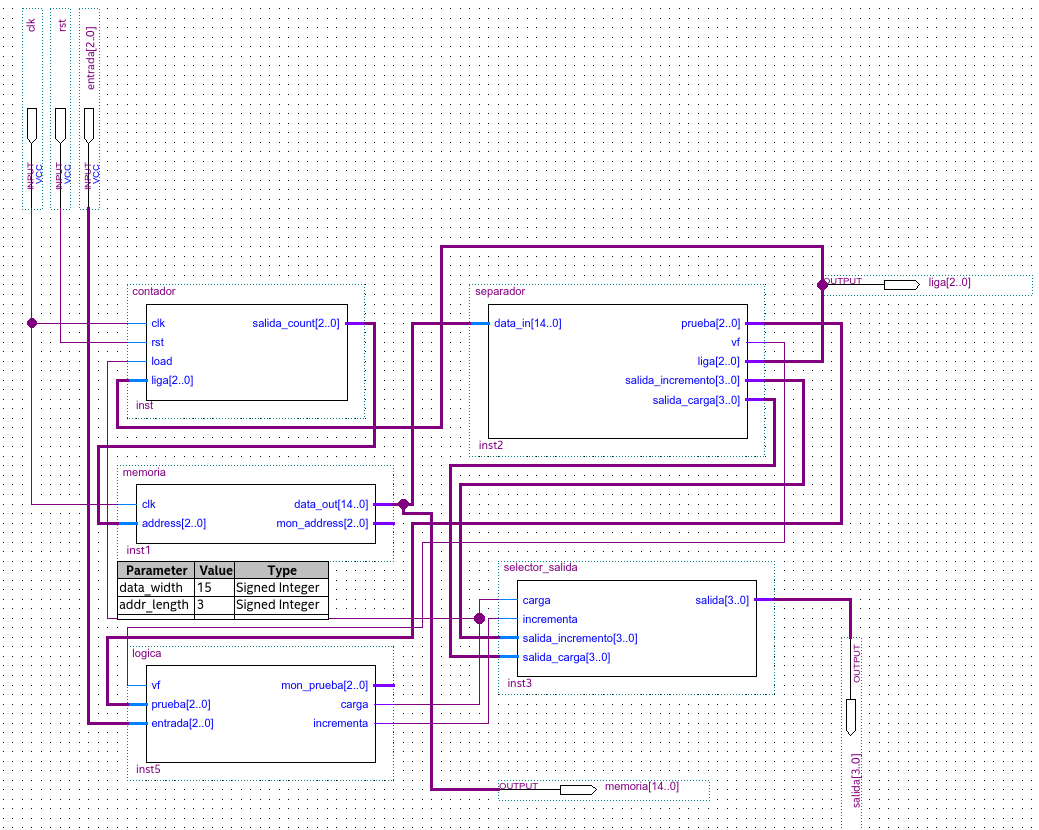
\includegraphics[width=\textwidth]{./img/dia}
    \caption{Diagrama}
\end{figure}



\subsection{Simulación}\label{sec:simulacion}
\begin{figure}[H]
  \centering
  \begin{subfigure}
    \centering
    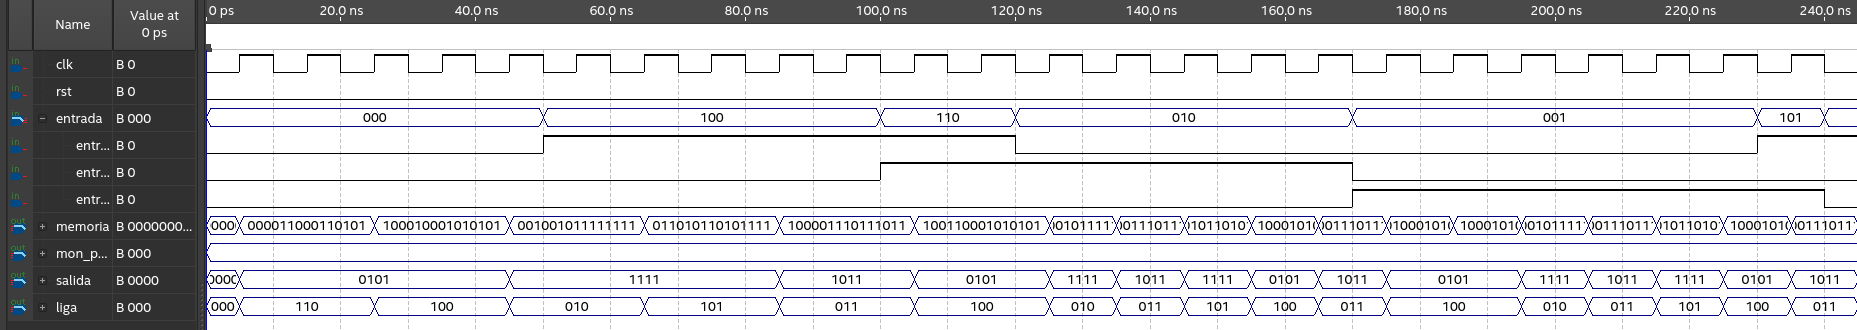
\includegraphics[width=\textwidth]{./img/sim1}
  \end{subfigure}

  \begin{subfigure}
    \centering
    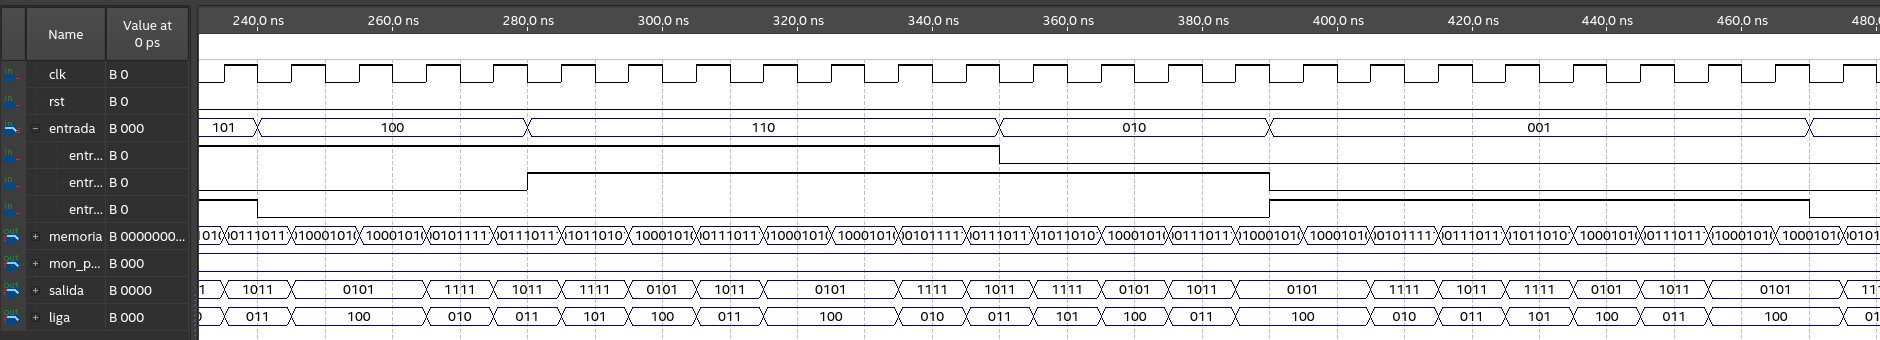
\includegraphics[width=\textwidth]{./img/sim2}
  \end{subfigure}
  \caption{Simulación}
  \label{fig:sim}
\end{figure}

\section{Conclusiones}
\label{sec:orgdab2190}

\subsection*{Monsalvo Bolaños Melissa Monserrat}\label{sec:mons-bolan-melissa}
Gracias a esta práctica pudimos implementar el desarrollo de una máquina de
estado usando memorias por direccionamiento implícito, esto requirió la
implementación de un contador y la modificación de la memoria para las salidas,
del mismo modo utilizamos variables nuevas como vf. En comparación con prácticas
pasadas está un poco más complicada.

\subsection*{Romero Andrade Cristian}\label{sec:romero-andr-crist}

Romero Andrade Cristian: En la práctica, el direccionamiento implícito se
implementó en VHDL, donde se desarrollaron los bloques que se muestran en la
Figura 1. La ventaja de este tipo de direccionamiento es que no se integra
colocando ninguna dirección de forma explícita, ya que la dirección se conoce en
el propio opcode los operandos a los que desea acceder o trabajar

\subsection*{Conclusiones en equipo}\label{sec:concl-en-equipo}

En la práctica se implementó el direccionamiento implícito en VHDL, donde se
desarrollaron los bloques de la figura 1, este tipo de direccionamiento tiene el
beneficio de no integrar poner ninguna dirección de forma explícita, ya que en
el propio código de operación se conoce la dirección de los operandos al que se
desea acceder o con el que se quiere operar.
\nocite{*}
\addcontentsline{toc}{section}{Referencias}
\printbibliography{}
\newpage{}

\listoftables{}
\listoffigures{}
\listoflistings{}
\end{document}
